\section{短视误差单调控制的死锁机理与严格局部极小有理数证书}\label{sec:obstruction}

\subsection{短视比例吸引投影的变分不等式与法锥锁死}
在传统安全导航框架中\cite{ames2017cbf,reis2021}，每台机器人的标称参考速度直接取为指向各自目标的比例吸引律 $\bu_i^{\mathrm{nom}}=-k_g\be_i=-k_g(\bp_i-\bg_i)$（$k_g>0$），全网经集中式安全滤波投影后的控制输入为 $\bu_G=\Pi_{\mathcal K_0(\bp)}(-k_g\be)$。由闭凸集 $\mathcal K_0(\bp)$ 上欧氏投影的一阶变分不等式可得：
\begin{equation}
 (\bu_G+k_g\be)^{\top}(\boldsymbol v-\bu_G)\ge 0,\qquad\forall\boldsymbol v\in\mathcal K_0(\bp).
 \label{eq:vi-proj}
\end{equation}
将始终属于安全输入集的零速度解 $\boldsymbol v=\boldsymbol 0\in\mathcal K_0(\bp)$ 代入式\eqref{eq:vi-proj}，即得原始位置误差函数 $W(\bp)$ 沿闭环轨迹的时间导数满足
\begin{equation}
 \dot W(\bp)=\be^{\top}\bu_G\le -\frac{1}{k_g}\norm{\bu_G}_2^2\le 0.
 \label{eq:W-descent}
\end{equation}
式\eqref{eq:W-descent}表明，只要安全集 $\mathcal K_0(\bp)$ 包含零速度，短视比例吸引安全控制器在结构上就强制要求全网总位置误差 $W(\bp(t))$ 沿轨迹单调不增。然而，单调不增并不意味着 $W(\bp(t))$ 能够衰减至零：当系统处于某个非目标构型（$\be\ne\boldsymbol 0$）时，一旦标称吸引向量 $-k_g\be$ 落入可行输入集在零输入处的法锥（Normal Cone）$N_{\mathcal K_0(\bp)}(\boldsymbol 0)=\{\boldsymbol w\in\mathbb R^{2N}:\boldsymbol w^{\top}\boldsymbol v\le 0,\ \forall\boldsymbol v\in\mathcal K_0(\bp)\}$\cite{rockafellar1970}，则任何非零安全速度都无法在一阶上减小 $W$，安全滤波器的唯一精确全局最优解即退化为零速度 $\bu_G=\boldsymbol 0$。此时即便底层分布式优化算法在当拍完全收敛至集中式最优解，系统仍会原地锁死。

\subsection{七机器人严格非目标局部极小定理与协同让路能垒}\label{subsec:seven-kkt}
文献中常将安全滤波器的死锁视为可通过微小扰动或局部负曲率逃离的不稳定鞍点\cite{reis2021,tan2024equilibria}。为从数学上严格证伪这一普适性假设，并揭示“构型空间存在宽裕安全可达路径、但任何要求 $\dot W\le 0$ 的控制器都会被彻底锁死在严格局部极小阱内”的机理，考察图\ref{fig:seven-geom}(a) 所示的七机器人平面双三角对称构型 $\bar\bp\in\mathbb R^{14}$（取安全距离 $\ds=1\ \mathrm m$，单机速度上限 $U=1/2\ \mathrm{m/s}$，矩阵每一列对应一台机器人的二维坐标）：
\begin{equation}
 \bar\bp^{\top}=\begin{bmatrix}
 -1 & -1/2 & -1/2 & 0 & 1/2 & 1/2 & 1\\
 0 & \sqrt{3}/2 & -\sqrt{3}/2 & 0 & \sqrt{3}/2 & -\sqrt{3}/2 & 0
 \end{bmatrix}.
 \label{eq:seven-config}
\end{equation}
在构型 $\bar\bp$ 中，$7$ 台机器人全员均可自由移动，相邻间距均为 $1\ \mathrm m$，共形成 $12$ 条恰好处于避碰边界（$d_{ij}=1\ \mathrm m$）的接触边集合 $\mathcal E_c=\{12,13,14,24,25,34,36,45,46,47,57,67\}$；外围五台机器人（$1,2,3,5,6$ 号）初始已处于各自目标位置（$\bg_i=\bar\bp_i,\be_i=\boldsymbol 0$），唯独位于正中心的机器人 $4$（坐标 $(0,0)$）与最右侧的机器人 $7$（坐标 $(1,0)$）需要互换位置（$\bg_4=\bar\bp_7,\bg_7=\bar\bp_4$）。

\begin{figure*}[htbp]
 \centering
 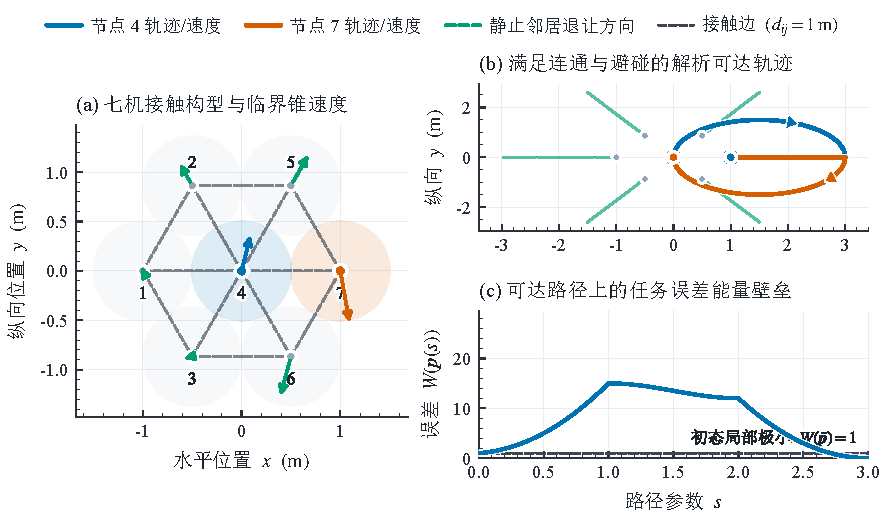
\includegraphics[width=\textwidth]{figures_zh/fig1_seven_geometry.pdf}
 \caption[七机器人严格局部极小构型与安全可达路径构造]{七机器人严格非目标局部极小构型与安全可达路径构造。(a) 式\eqref{eq:seven-config}的双三角对称接触构型、12 条初始接触边与式\eqref{eq:certificate-primal}的临界锥最优速度见证向量；(b) 先均匀放大 $3$ 倍、节点 $4$ 与 $7$ 沿相反半圆交换位置、再均匀缩回的解析安全可达轨迹；(c) 沿可达路径的任务误差曲线 $W(\bp(s))$（任何安全可达轨迹必须先越过高于初态 $W(\bar\bp)=1$ 的能量壁垒）。}
 \label{fig:seven-geom}
\end{figure*}

\begin{theorem}[七机器人对称接触构型的严格局部极小有理数证书与能量壁垒]\label{thm:seven-kkt}
对于式\eqref{eq:seven-config}定义的七机器人位置互换任务（$\ds=1\ \mathrm m,\lr=5/2,R_c=10\ \mathrm m$），成立如下精确结论：
\begin{enumerate}
 \item \textbf{一阶平稳性与二阶临界锥严格正定性：} 在初态 $\bar\bp$ 处，$W(\bar\bp)=1$，$\lambda_2(\bL(\bar\bp))>5/2$，且 $\nabla W(\bar\bp)=\frac12\nabla h_{47}^{\mathrm{col}}(\bar\bp)$，故 $\bu_G=\boldsymbol 0$ 为式\eqref{eq:central-proj}的精确最优解。记完整临界方向锥为 $\mathcal C=\{\boldsymbol v\in\mathbb R^{14}:\bar\bp_{ij}^{\top}(\boldsymbol v_i-\boldsymbol v_j)\ge 0\ (\forall\{i,j\}\in\mathcal E_c),\ v_{4x}=v_{7x}\}$，拉格朗日 Hessian 为 $\boldsymbol H_L=\I_{14}-(\boldsymbol b_{47}\boldsymbol b_{47}^{\top})\otimes\I_2$，则在 $\mathcal C$ 上恒有精确有理数下界
 \begin{equation}
\begin{split}
  \min_{\boldsymbol v\in\mathcal C,\ v_{4y}-v_{7y}=1}\norm{\boldsymbol v}_2^2&=\frac{515}{496}>1,\\
  \boldsymbol v^{\top}\boldsymbol H_L\boldsymbol v&\ge\frac{19}{515}\norm{\boldsymbol v}_2^2>0\quad(\forall\boldsymbol v\in\mathcal C\setminus\{\boldsymbol 0\}).
\end{split}
  \label{eq:critical-hessian}
 \end{equation}
 \item \textbf{有限邻域球面二次能量壁垒与严格内部开球陷阱：} 对任意满足全部机间避碰约束（$d_{ij}(\bar\bp+\boldsymbol\delta)\ge 1$）的非零位置扰动 $0<\norm{\boldsymbol\delta}_2\le\frac1{200}$，恒有显式能量上升下界
 \begin{equation}
  W(\bar\bp+\boldsymbol\delta)-W(\bar\bp)\ge\frac{1}{100}\norm{\boldsymbol\delta}_2^2>0.
  \label{eq:finite-barrier}
 \end{equation}
 进一步，对初态与目标均严格位于安全集内部（无初始接触）的微扰任务 $\bp_0=(1+10^{-8})\bar\bp,\bg_\tau=(1+10^{-6})\bg$，以 $\bp_0$ 为中心、半径 $\rho=\frac1{4\times 10^8}$ 的开球 $B_\rho(\bp_0)\subset\operatorname{int}(\mathcal S)$ 内任一初态出发的连续安全轨迹，若满足 $\dot W_\tau\le 0$，则永远被困于球面 $\norm{\bp-\bar\bp}_2=\frac1{200}$ 内部（球面壁垒 $W_\tau(\bar\bp+\boldsymbol\delta)-W_\tau(\bar\bp)\ge\frac{19}{8\times 10^7}>W_\tau(\bp)-W_\tau(\bar\bp)$），无法到达球外目标 $\bg_\tau$。
 \item \textbf{全局安全与谱连通可达性：} 存在一条显式连续分段光滑路径 $\bp(s)\ (s\in[0,3])$ 连接初态与目标，全程严格满足避碰距离 $d_{ij}(s)\ge 1\ \mathrm m$ 以及代数连通度下界 $\lambda_2(\bL(\bp(s)))\ge\frac{1792}{625}=2.8672>\frac52$。
\end{enumerate}
\end{theorem}
\begin{proof}
（1）在 $\bar\bp$ 处，$\be_4=(-1,0)^{\top},\be_7=(1,0)^{\top}$，其余 $\be_i=\boldsymbol 0$；接触边 $\{4,7\}$ 的障碍梯度在节点 $4,7$ 分量上分别为 $2(\bar\bp_4-\bar\bp_7)=(-2,0)^{\top}$ 与 $2(\bar\bp_7-\bar\bp_4)=(2,0)^{\top}$，故取乘子 $\lambda_{47}=\frac12$、其余乘子为 $0$ 即满足平稳性 $\nabla W(\bar\bp)-\frac12\nabla h_{47}^{\mathrm{col}}(\bar\bp)=\boldsymbol 0$。沿临界方向 $\boldsymbol v\in\mathcal C$，因 $v_{4x}=v_{7x}$，有 $\boldsymbol v^{\top}\boldsymbol H_L\boldsymbol v=\norm{\boldsymbol v}_2^2-|v_{4y}-v_{7y}|^2$。将速度按有理数坐标缩放表示为 $\boldsymbol v_i=(z_{ix},\sqrt{3}z_{iy})^{\top}$ 并堆叠为 $\boldsymbol z\in\mathbb R^{14}$，令对角矩阵 $Q_c=\diag(1,3,\dots,1,3)$，则 $\norm{\boldsymbol v}_2^2=\boldsymbol z^{\top}Q_c\boldsymbol z$。定义有理数接触矩阵 $(G_c\boldsymbol z)_{ij}=\bar p_{ij,x}(z_{ix}-z_{jx})+\sqrt{3}\bar p_{ij,y}(z_{iy}-z_{jy})$ 与等式矩阵 $E_c\boldsymbol z=[z_{4x}-z_{7x},\,z_{4y}-z_{7y}]^{\top}$，考察凸二次规划 $\min\boldsymbol z^{\top}Q_c\boldsymbol z\ \text{s.t.}\ G_c\boldsymbol z\ge\boldsymbol 0,\,E_c\boldsymbol z=(0,1)^{\top}$。构造精确有理数原始解见证 $Z_*\in\mathbb Q^{7\times 2}$ 与对偶乘子 $(\boldsymbol\mu,\boldsymbol\nu)$：
\begin{equation}
\begin{split}
 Z_*^{\top}&=\frac{1}{496}{\setlength{\arraycolsep}{2.5pt}\begin{bmatrix}
 -15 & -132 & -105 & 90 & 177 & -105 & 90\\
 15 & 132 & -15 & 206 & 177 & -225 & -290
 \end{bmatrix}},\\
 \mu_{13}&=\tfrac{15}{248},\ \mu_{24}=\tfrac{33}{62},\ \mu_{36}=\tfrac{15}{62},\ \mu_{45}=\tfrac{177}{248},\ \mu_{67}=\tfrac{225}{248},\\
 \boldsymbol\nu&=\big[\tfrac{135}{496},\,\tfrac{1545}{496}\big]^{\top},
\end{split}\label{eq:certificate-primal}
\end{equation}
其余接触边乘子为 $0$。直接由有理数算术核验可知，$\boldsymbol z_*=\col((Z_*)_{1,:}^{\top},\dots,(Z_*)_{7,:}^{\top})$ 满足原始可行性 $G_c\boldsymbol z_*\ge\boldsymbol 0,E_c\boldsymbol z_*=(0,1)^{\top}$、互补松弛 $\boldsymbol\mu^{\top}G_c\boldsymbol z_*=0$ 及平稳性条件 $Q_c\boldsymbol z_*=G_c^{\top}\boldsymbol\mu+E_c^{\top}\boldsymbol\nu$，最优值为 $\boldsymbol z_*^{\top}Q_c\boldsymbol z_*=\frac{1545}{496}$。由凸二次规划强对偶性并除以纵向缩放因子 $(\sqrt{3})^2=3$，即得 $\min_{\boldsymbol v\in\mathcal C,v_{4y}-v_{7y}=1}\norm{\boldsymbol v}_2^2=\frac{1545}{3\times 496}=\frac{515}{496}>1$（由上下反射对称性对 $v_{4y}-v_{7y}=-1$ 同样成立），从而按齐次性得 $\boldsymbol v^{\top}\boldsymbol H_L\boldsymbol v\ge(1-\frac{496}{515})\norm{\boldsymbol v}_2^2=\frac{19}{515}\norm{\boldsymbol v}_2^2$，即式\eqref{eq:critical-hessian}。

（2）设 $\boldsymbol\delta\in\mathbb R^{14}$ 满足 $0<R:=\norm{\boldsymbol\delta}_2\le\frac1{200}$ 及避碰条件 $\norm{\bar\bp_{ij}+\boldsymbol\delta_i-\boldsymbol\delta_j}_2^2\ge 1\ (\forall\{i,j\}\in\mathcal E_c)$。记 $z=\delta_{4x}-\delta_{7x},t=\delta_{4y}-\delta_{7y}$，则 $W(\bar\bp+\boldsymbol\delta)-W(\bar\bp)=\frac12 R^2-z$。若 $z\le 0$，式\eqref{eq:finite-barrier}显然成立；下设 $z>0$。每条接触边的非线性避碰条件展开为 $\bar\bp_{ij}^{\top}(\boldsymbol\delta_i-\boldsymbol\delta_j)\ge -\frac12\norm{\boldsymbol\delta_i-\boldsymbol\delta_j}_2^2\ge -R^2$。将有理缩放坐标下的平稳性恒等式 $Q_c\boldsymbol z_*=G_c^{\top}\boldsymbol\mu+E_c^{\top}\boldsymbol\nu$ 与缩放扰动 $\tilde{\boldsymbol\delta}$ 作内积，利用 $\boldsymbol\mu\ge\boldsymbol 0$、$\sum_{\{i,j\}\in\mathcal E_c}\mu_{ij}=\frac{609}{248}=:S$、$c=\frac{1545}{496}$ 及 Cauchy–Schwarz 不等式，可得 $\frac{c}{\sqrt{3}}|t|\le\sqrt{c}R+SR^2$。因 $S/\sqrt{c}\le\frac32$，平方整理得 $t^2\le\frac{496}{515}R^2(1+\frac32 R)^2$。又由交换边 $\{4,7\}$ 的避碰条件 $(-1+z)^2+t^2\ge 1\implies 2z\le z^2+t^2$，结合 $z\le\sqrt{2}R<1$ 与 $t^2\le 2R^2$ 可得 $z\le 2R^2$，代入 $2z\le z^2+t^2$ 得 $z\le 2R^4+\frac12 t^2$。因此
\begin{equation}
\begin{split}
 W(\bar\bp+\boldsymbol\delta)-W(\bar\bp)&=\frac12 R^2-z\\
 &\ge\frac{R^2}{2}\left[1-\frac{496}{515}\Big(1+\frac32 R\Big)^2-4R^2\right]\\
 &\ge\frac{1}{100}R^2,\qquad\forall R\in\Big(0,\frac1{200}\Big].
\end{split}
\end{equation}
对于严格内部微扰版本 $\bp_0=(1+10^{-8})\bar\bp,\bg_\tau=(1+10^{-6})\bg$，在球面 $\norm{\boldsymbol\delta}_2=r=\frac1{200}$ 上由 $\norm{\bg}_2=\sqrt{6}<\frac52$ 得 $W_\tau(\bar\bp+\boldsymbol\delta)-W_\tau(\bar\bp)=W(\bar\bp+\boldsymbol\delta)-W(\bar\bp)-\tau\bg^{\top}\boldsymbol\delta\ge\frac{r^2}{100}-\frac52\tau r=\frac{19}{8\times 10^7}$，而在开球 $B_\rho(\bp_0)$ 内最大误差增量严格低于该球面壁垒，故任何单调不增的安全轨迹均无法穿过球面 $\norm{\bp-\bar\bp}_2=\frac1{200}$。

（3）构造图\ref{fig:seven-geom}(b) 所示的三阶段路径：$s\in[0,1]$ 时全体位置均匀放大至 $3\bar\bp$；$s\in[1,2]$ 时外围五机保持在 $3\bar\bp_i$，节点 $4$ 与 $7$ 绕中心 $(3/2,0)$ 沿半径 $3/2$ 的相反半圆交换位置；$s\in[2,3]$ 时全体位置从 $3\bg$ 均匀缩回 $\bg$。在半圆交换阶段，节点 $4,7$ 间距恒为 $3\ge 1$，外围五机到圆心 $(3/2,0)$ 的距离平方最小为 $\frac{27}{4}>(\frac32+1)^2=\frac{25}{4}$，故全程满足 $d_{ij}(s)\ge 1$。全程任意两机最大距离不超过 $6\ \mathrm m$，由式\eqref{eq:poly-channel}知每条完全图边权满足 $w_{ij}(s)\ge(1-\frac{36}{100})^2=\frac{256}{625}$，故 $\lambda_2(\bL(\bp(s)))\ge 7\times\frac{256}{625}=\frac{1792}{625}>\frac52$。
\end{proof}

\begin{remark}[七机器人见证启发的协同控制构造]\label{rem:two-conditions}
定理\ref{thm:seven-kkt}及见证式\eqref{eq:certificate-primal}启发以下两项控制构造。它们描述本文采用的局部脱困机制，不构成任意重排任务的全局充要条件：
\begin{enumerate}
 \item \textbf{待互换机器人的侧向破对称标称驱动：} 在临界锥最优错开方向式\eqref{eq:certificate-primal}中，中心机器人 $4$ 与右侧机器人 $7$ 必须产生相反的纵向（垂直于目标误差 $\be_4,\be_7$）速度分量 $z_{4y}=+\frac{206}{496}>0$ 与 $z_{7y}=-\frac{290}{496}<0$（图\ref{fig:seven-geom}(a) 蓝色与橙色箭头）。若标称控制器仅提供沿 $\be_i$ 方向的径向吸引，则系统永远停留在 $v_{4y}-v_{7y}=0$ 的共线死锁子空间内。
 \item \textbf{外围静止邻居经由动态配额让渡实现的协同退让：} 式\eqref{eq:certificate-primal}表明，当机器人 $4$ 与 $7$ 沿纵向错开时，周围五台原本已处于各自目标位置（$\be_j=\boldsymbol 0$）的静止邻居必须同步产生非零向外退让速度（如 $(Z_*)_{2,:}=\frac1{496}[-132,132]$、$(Z_*)_{5,:}=\frac1{496}[177,177]$，见图\ref{fig:seven-geom}(a) 翠绿色箭头），该运动通过接触边上的严格正对偶乘子 $\mu_{24},\mu_{45},\mu_{67}>0$ 实现力学传递。若安全滤波器采用静态配额平摊（固定各节点在避碰行上的份额为零），则 $\be_j=\boldsymbol 0$ 的静止邻居保持 $\bu_j=\boldsymbol 0$，接触约束直接把机器人 $4$ 与 $7$ 的纵向错开分量截断为零。
\end{enumerate}
上述两项机理直接决定了第\ref{sec:method}节的 EGP-NPA 控制架构设计：由等变图网络强化学习策略为受阻移动机器人提供手性侧向绕行标称速度，并由闭邻域块 NPA 滤波器的动态零和份额转移驱动外围静止邻居协同退让。
\end{remark}
